\documentclass [9 pt]{article}
\usepackage[margin = 1in]{geometry}
\usepackage{amsfonts}
\usepackage{amsthm}
\usepackage{bbm}
\usepackage{amsmath}
\usepackage{arydshln}
\usepackage[utf8]{inputenc}
\usepackage{graphicx}
\usepackage{enumerate}
\usepackage{color}
\usepackage[dvipsnames]{xcolor}
\usepackage{graphicx}
\graphicspath{ {./images/} }
\usepackage{tikz}
\usepackage{xcolor}
\usepackage{listings}
\usepackage{color}
\usepackage{algorithm}
\usepackage{algpseudocode}
\usepackage{tikz}
\usepackage{booktabs}
\usepackage[framemethod = tikz]{mdframed}

\definecolor{dkgreen}{rgb}{0,0.6,0}
\definecolor{gray}{rgb}{0.5,0.5,0.5}
\definecolor{mauve}{rgb}{0.58,0,0.82}


\lstset{
  language=Matlab,
  basicstyle=\ttfamily,               
  numbers=left,                  
  stepnumber=1,                  
  numbersep=5pt,                  
  backgroundcolor=\color{white}, 
  showspaces=false,              
  showstringspaces=false,        
  showtabs=false,                
  tabsize=2,                     
  captionpos=b,                  
  breaklines=true,               
  breakatwhitespace=true,         
  title=\lstname,
  numberstyle=\tiny\color{Black},
  keywordstyle=\color{BrickRed},
  commentstyle=\color{dkgreen},
  stringstyle=\color{mauve},  
}

\theoremstyle{definition}
\newtheorem{problem}{Problem}
\newtheorem{theorem}{Theorem}
\newtheorem*{corollary}{Corollary}
\newtheorem{proposition}[theorem]{Proposition}
\newtheorem{lemma}[theorem]{Lemma}
\newtheorem{conjecture}[theorem]{Conjecture}

\newtheorem{definition}[theorem]{Definition}
\newtheorem{remark}[theorem]{Remark}
\newtheorem{example}[theorem]{Example}


\usepackage{fancyhdr}
\pagestyle{fancy}
\lhead{Yuhao Wu \quad 260711365} 
\rhead{\bfseries COMP 350 Final Review 5}
\cfoot{\thepage}
\renewcommand{\headrulewidth}{0.4pt}
\renewcommand{\footrulewidth}{0.4pt}


\setlength{\parindent}{0pt}


\begin{document}

\title{Numerical Integration (20 points)}
\date{2018-11-30}
\author{Name: Yuhao Wu\\
ID Number: 260711365
}
\maketitle

\section*{Rectangle Rule:}
Partition $[a, b]$ into $n$ equal subintervals $[x_i, x_{i+1}], i = 0, 1, 2, \ldots , n$ all with width $h = \dfrac{b - a}{n}$\\
\\
The area of the rectangle over $[x_i, x_{i+1}]$ is 
$$ h \cdot f(x_i) = h \cdot f(a + i \cdot h) $$
So, the \textbf{ total area } of $n$ rectangle panels is 
$$I_R = h \cdot \sum_{i = 0}^{n - 1} f(a + i \cdot h)$$

\begin{theorem}
	Let $f'$ be continuous on $[a, b]$. Then for some $z \in [a, b]$
	$$I - I_R = \dfrac{1}{2} (b - a)\cdot h \cdot f'(z) = O(h) $$
\end{theorem}
\begin{proof}
	First, we show that when $h = b - a$ the results holds, which is to prove that 
	\begin{equation}
		I - I_R = \dfrac{1}{2} (b - a)^2 \cdot f'(z) = O(h)
	\end{equation}
	
	$$\Bigg[ Taylor\ Theorem: f(x) = f(a) + \dfrac{f'(a)}{1!}(x - a) + \dfrac{f''(a)}{2!}(x - a)^2 + \ldots + \dfrac{f^{(n)} (a)}{n!}(x - a)^n + R_n(x)  \Bigg]$$
	
	
	For any $x \in [a, b]$, we do Taylor Expansion at $a$, then we have:
	\begin{equation}
	f(x) = f(a) + (x - a) f'(z_x)\quad\  where \ z_x \in [a, b] 	
	\end{equation} 
	
	Then: 
	\begin{align*}
		I - I_R 
		&= \int_{a}^{b} f(x)\ dx - f(a)\cdot (b - a)\\
		&= \int_{a}^{b} f(x)\ dx - \int_{a}^b f(a)\ dx \quad \text{As $f(a)$ is a constant}  \\
		&= \int_{a}^b [f(x) - f(a)]\ dx \\
		&= \int_{a}^b (x - a) f'(z_x)\ dx \quad \quad \text{use equation(2)} \\
		&= f'(z) \cdot \int_{a}^b (x - a)\ dx \quad z \in [a, b] \quad \text{ (MVT for integral) }\\
		&= \dfrac{1}{2}(b - a)^2 f'(z)
	\end{align*}
	
	Now suppose that $[a, b]$ is divided into $n$ equal subinterval by $x_0, x_1, x_2, \ldots , x_n$ with panel width $h = \dfrac{b - a}{n}$\\
	\\
	Applying above results to each of the subinterval $[x_i, x_{i+1}]$, then we have:
	\begin{equation}
		\int_{x_i}^{x_{i+1}} f(x)\ dx - f(x_i)\cdot h = \dfrac{1}{2} (x_{i + 1} - x_{i})^2 f'(z_i) = \dfrac{1}{2} h^2\cdot f'(z_i)\quad \text{ for some } z_i \in [x_i, x_{i+1}]
	\end{equation} 
	
	So, we have 
	\begin{align*}
		I - I_R 
		&= \int_{a}^{b} f(x)\ dx - h\cdot \sum_{i = 0}^{n - 1}f(x_i)\\
		&= \sum_{i = 0}^{n - 1} \int_{x_i}^{x_{i+1}} f(x)\ dx - h \cdot \sum_{i = 0}^{n - 1}f(x_i)\\
		&= \sum_{i = 0}^{n - 1} \dfrac{1}{2}h^2 \cdot f'(z_i)\\
		&= n \cdot \dfrac{1}{2}h^2 \cdot f'(z) \quad \quad \text{MVT for sum} \\
		&= \dfrac{1}{2} (b - a) h \cdot f'(z)
	\end{align*}
	
\end{proof}

\section*{Midpoint Rule:}
The Midpoint Rule:
$$ I_M = h \sum_{i = 0}^{n - 1} f\Big[ a + ( i + \dfrac{1}{2} h)  \Big] \quad where\ h = \dfrac{b - a}{n} $$
\textbf{Error Analysis:}
It can be proven for some $z \in [a, b]$, we have
$$I - I_M = \dfrac{1}{24} (b - a) h^2 f''(z) = O(h^2) $$

\section*{Trapezoid Rule:}
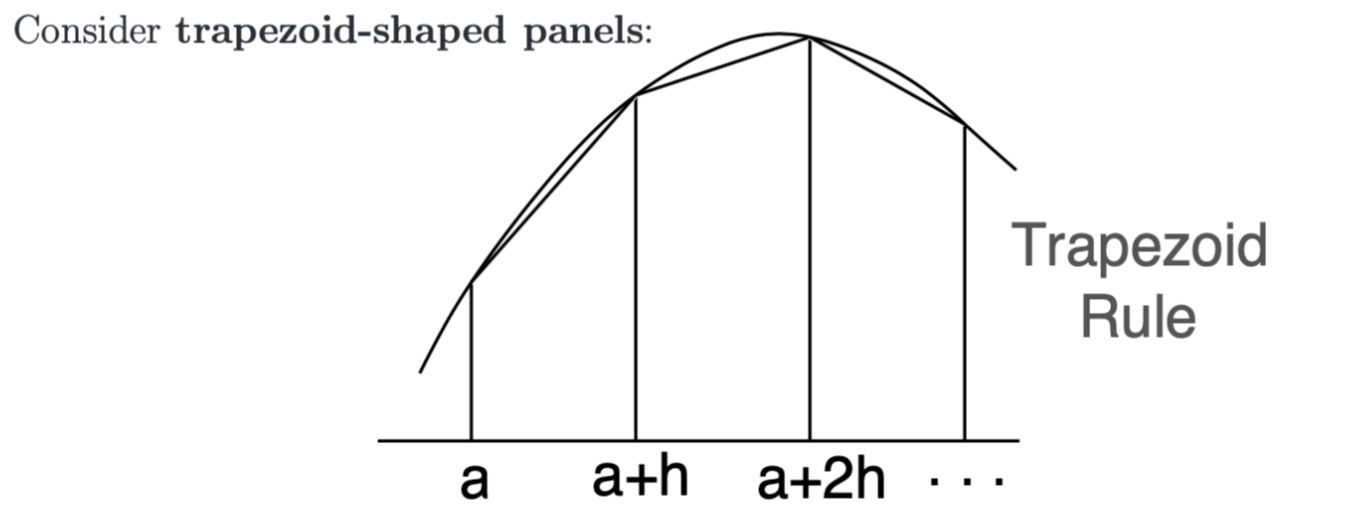
\includegraphics[scale = 0.5]{1}\\
For the first panel, the area is $\dfrac{1}{2}\cdot h \cdot \Big(  f(a) + f(a + h) \Big)$\\
For the second panel, the area is $\dfrac{1}{2}\cdot h \cdot  \Big( f(a + h) + f(a + 2 \cdot h) \Big)$\\
As all the points are added up twice except for the left-most and right-most points:
$$ I_T = \dfrac{1}{2} \cdot h \Big[ f(a) + f(b) \Big] + h \cdot \sum_{i = 1}^{n - 1} f(a + i\cdot h) \quad with\ h = \dfrac{b - a}{n}  $$
\textbf{Error Analysis:}\\
It can be shown that for some $z \in [a, b]$
$$ I - I_T = - \dfrac{1}{12} (b - a) \cdot h^2 f''(z) = O(h^2) $$

\subsection*{Recursive Trapezoid Rule:}
Suppose that $[a, b]$ is divided into $2^n$ equal subintervals. Then the trapezoid rule is:
$$ I_T(2^n) = \dfrac{1}{2} \cdot h \Big[ f(a) + f(b) \Big] + h \sum_{i = 1}^{2^n - 1} f(a + i\cdot h)\quad where\ h = \dfrac{b - a}{2^n} $$
The trapezoid rule for $2^{n - 1}$ equal subintervals is:
$$ I_T(2^{n - 1}) = \dfrac{1}{2} \widehat{h}\cdot \Big[ f(a) + f(b) \Big] + \widehat{h}\cdot \sum_{i = 1}^{2^{n-1} - 1} f(a + i\cdot \widehat{h})\quad where\ \widehat{h} = \dfrac{b - a}{2^{n - 1}} = 2 \cdot h $$

\begin{align*}
	I_T(2^n)
	&= \dfrac{1}{2} h \cdot \big[ f(a) + f(b) \big] + h \sum_{i = 1}^{2^n - 1} f(a + i\cdot h) + \dfrac{1}{2} \cdot I_T(2^{n - 1}) - \dfrac{1}{4}\widehat{h}\cdot \Big[ f(a) + f(b) \Big] - \dfrac{1}{2} \widehat{h}\cdot \sum_{i = 1}^{2^{n-1} - 1} f(a + i\cdot \widehat{h}) \\
	&= \dfrac{1}{2} \cdot I_T(2^{n - 1}) + h \sum_{i = 1}^{2^n - 1} f(a + i\cdot h) - \dfrac{1}{2} \widehat{h}\cdot \sum_{i = 1}^{2^{n-1} - 1} f(a + i\cdot \widehat{h}) \\
	&=  \dfrac{1}{2} \cdot I_T(2^{n - 1}) + h \sum_{i = 1}^{2^n - 1} f(a + i\cdot h) - h \cdot \sum_{i = 1}^{2^{n-1} - 1} f(a + i\cdot 2h) \\
	&\text{the second term is all the $i$ from 1 to $2^n - 1$} \quad \text{the third term is all the even $i$ from 1 to $2^n - 1$}\\
	&= \dfrac{1}{2} \cdot I_T(2^{n - 1}) + h \cdot \sum_{i = 1}^{2^{n-1} } f\Big(a + (2i - 1)\cdot h\Big) \\
\end{align*}

\textbf{Why we need Recursive:}
\begin{mdframed}
	\begin{itemize}
		\item After computing $I_T(2^{n - 1})$, we can compute $I_T(2^n)$ by recursive formula without reevaluating $f$ at some old points
		\item We can use the recursive formula to determine how many iterations we need by\\ $ |I_T(2^n) - I_T(2^{n - 1}) |  < \delta$
	\end{itemize}
\end{mdframed}

\section*{Simpson's Rule:}
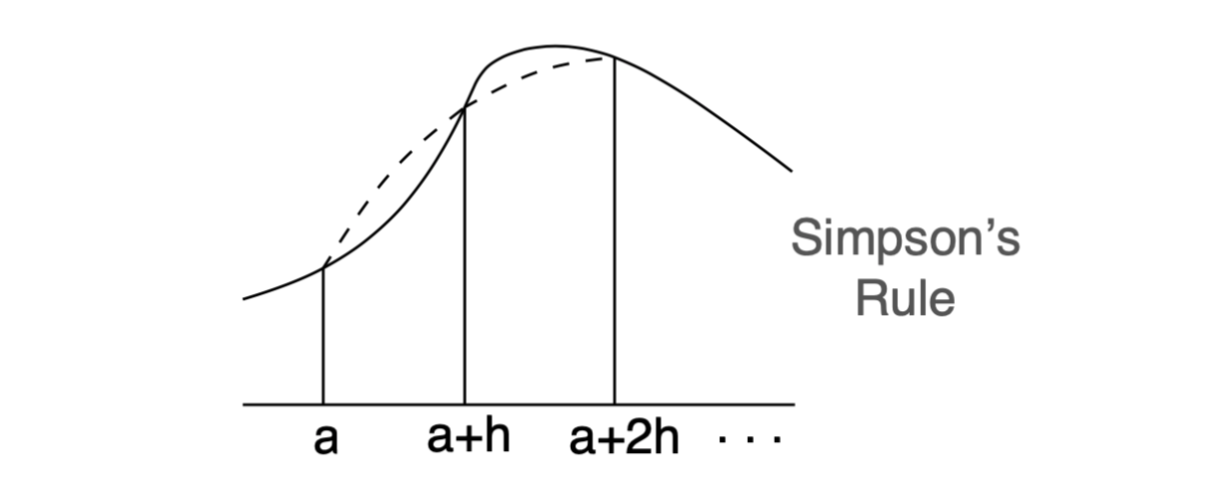
\includegraphics[scale = 0.5]{2}\\
There are an even number of panels with width $h=\dfrac{b-a}{n}$. \\
The top boundary of the first pair of panels is the quadratic which interpolates $(a, f(a)), (a+h, f(a+h)), (a+ 2h, f(a+ 2h))$. \\
The next interpolates $(a+ 2h, f(a+ 2h)),(a+ 3h, f(a+ 3h)), (a+ 4h, f(a+ 4h))$, and so on.\\
\\
The area of the first 2 panels can be shown to be:
$$ \dfrac{h}{3}\Big[ f(a) + 4f(a + h) + f(a + 2h) \Big] $$.
For the total area, we sum them up:
\begin{align*}
	&\dfrac{h}{3}\Big[ f(a) + 4f(a + h) + f(a + 2h) \Big] \\
	&\dfrac{h}{3}\Big[ f(a+2h) + 4f(a + 3h) + f(a + 4h) \Big] \\
	&\vdots\\
	&\dfrac{h}{3}\Big[ f(b- 2h) + 4f(b - h) + f(b) \Big] \\
\end{align*}
Then we have \textbf{Simpson's Rule:}
$$I_S  = \dfrac{h}{3} \Bigg[ f(a) + 4\cdot f(a + h) + 2 \cdot f(a + 2h) + 4f(a + 3h) + 2 f(a + 4h) + \ldots + f(b) \Bigg] $$
As it is divided into $n = 2k$ subintervals, we can rewrite it as:
$$ I_S  = \dfrac{h}{3} \Bigg[ f(a) + f(b) +  4\cdot \sum_{i = 0}^{k - 1} f\Big(a + (2i + 1) \cdot h\Big)  + 2\cdot \sum_{i = 1}^{k - 1} f\Big(a + 2i\cdot h\Big) \Bigg] $$
\\
\textbf{Error Analysis:}\\
It can be shown for some $z \in [a, b]$:
$$I - I_S = - \dfrac{1}{180} \cdot (b - a)\cdot h^4\cdot f^{(4)}(z) = O(h^4) $$
\textbf{Question:}\\
What is the highest degree polynomial for which the rule is \textbf{exact} in general?
\begin{mdframed}
	The highest degree is 3.\\
	As for polynomial with degree 3,  $f^{(4)}(z)$ is always 0, which tells us the error is always 0.
\end{mdframed}



\newpage
\section*{Adaptive Method:}
\textbf{Question: Why do we need Adaptive Method?}
\begin{mdframed}
	A function may vary rapidly on some parts of the interval $[a, b]$, but vary little on other parts. It is not very efficient to use the same panel width $h$ everywhere on $[a, b]$. But on the other hand, we don't know in advance on which part of the integral $f$ varies rapidly. So, we need an adaptive integration method.
\end{mdframed}

\textbf{Basic Idea:}
\begin{mdframed}
	The basic idea is we divide $[a, b]$ into 2 subintervals and then decide whether each of them is to be divided into more subintervals. This procedure is continued until some specified accuracy is obtained throughout the whole interval $[a, b]$.
\end{mdframed}

\textbf{Basic Framework:}
\begin{algorithm}
\caption{Adaptive Method:}
\begin{algorithmic}[1]
\State Input: $f(x)\quad a, b$, \quad the tolerance $\delta$, \ldots
	\\
	\State Compute the integral from $a$ and $b$ in two ways
	\State call the values $I_1$ and $I_2$ separately (Assume $I_2$ is better than $I_1$)
	\State Estimate the error in $I_2$ based on $|I_2 - I_1|$
	\\
	\If{$| \text{ the Estimated Error } |\leq \delta$ }
		\State $numI = I_2 + \text{ the Estimated Error }$
	\Else
		\State $c = \dfrac{a + b}{2}$
		\State $numI = adapt(f, a, c, \dfrac{\delta}{2}, \ldots) + adapt(f, c, b, \dfrac{\delta}{2}, \ldots )$
	\EndIf
\end{algorithmic}
\end{algorithm}




\newpage
\section*{Gaussian Quadrature Rules:}
Unlike previous integration rules which choose equally spaced nodes for evaluation, Gaussian Quadrature rules choose the nodes $x_0, x_1, \ldots, x_n$ and coefficients $A_0, A_1, \ldots, A_n$ (which are also called weights) to minimize the expected error obtained in the approximation:
$$ \int_{a}^{b} f(x)\ dx \approx \sum_{i = 0}^{n} A_i f(x_i) $$\\
\\
To measure this accuracy, we assume that the best choice of theses values is that which produces the exact result for the largest class of polynomials.\\
\\
Derive for the case  $n = 1$
\begin{mdframed}
	$n = 1$, then we have:
	$$ \int_{-1}^1 f(x)\ dx = A_0 f(x_0) + A_1\cdot f(x_1) $$
	Suppose that $f(x) = x^j \quad j = 0, 1, 2, 3$
	$$ \int_{-1}^{1} x^j\ dx = \dfrac{1}{j + 1} x^{j + 1}\bigg|^1_{-1} $$
	Then we can have the four equations:
	\begin{align*}
		2 &= A_0 + A_1 \quad\quad\quad\quad\quad (1)\\
		0 &= A_0\cdot x_0 + A_1 \cdot x_1 \quad\quad\quad\quad\quad  (2)\\
		\dfrac{2}{3} &= A_0 \cdot x_0^2 + A_1 \cdot x_1^2 \quad\quad\quad\quad\quad  (3)\\
		0 &= A_0\cdot x_0^3 + A_1 \cdot x_1^3 \quad\quad\quad\quad\quad  (4)
	\end{align*}
	From Equation(2), we know that $A_0\cdot x_0 = - A_1 \cdot x_1$, we use this into Equation(4), which gives us:
	$$ A_1 \cdot x_1^3 - A_1 \cdot x_1 \cdot x_0^2 = 0 \implies A_1\cdot x_1 \cdot (x_1^2 - x_0^2) = 0 $$
	It is impossible for $A_1 \cdot x_1 = 0$, otherwise according to Equation(2), $A_0 \cdot x_0 = 0$ contradicts with Equation(3).\\
	\\
	Thus we have $x_1^2 = x_0^2$. It is also impossible for $x_1 = x_0 $(We have shown $A_1 \cdot x_1 \neq 0$). Otherwise, we will imply that $A_0 + A_1 = 0 $ from Equation(2), which contradicts with Equation(1).\\
	\\
	Then, we can say that $x_1 = - x_2 \implies A_0 = A_1  = 1 \implies x_0 = \dfrac{1}{\sqrt{3}}, x_1 = - \dfrac{1}{\sqrt{3}}$\\
	\\
	Thus, we have:
	$$ \int_{-1}^1 f(x)\ dx = 1 \cdot f(\dfrac{1}{\sqrt{3}}) + 1\cdot f( - \dfrac{1}{\sqrt{3}}) $$

\end{mdframed}

\newpage
\textbf{Question:}\\
What is the highest degree of polynomials for 
\begin{equation}
	\int_{a}^{b} f(x)\ dx = \sum_{i = 0}^n A_i \cdot f(x_i)
\end{equation} 
holds by choosing $x_i, i = 0, 1, 2, \ldots , n$
\begin{mdframed}
	Take $f(x) = x^j,\quad j = 0, 1, \ldots , m$\\
	$$\int_{a}^{b} x^j \ dx = \sum_{i = 0}^{n} A_i \cdot x_i^j \quad\quad j = 0, 1, \ldots , m	$$
	From above, we know there are $m + 1$ equations.\\
	From Equation(4), we know that there are $A_0, x_0, A_1, x_1, \ldots , A_n, x_n$, total $2n + 2$ unknowns.\\
	\\
	Thus, we have $m+1 \leq 2n + 2 \implies m \leq 2n + 1$\\
	\\
	For any polynomial $f(x)$ of degree $\leq 2n+1$.\\
	We can do linear combinations:
	$$f(x) = c_0 + c_1\cdot x + \ldots + c_{2n+1}\cdot x^{2n+1}$$
	\begin{align*}
		\int_{a}^{b} f(x)\ dx 
		&= \sum_{j = 0}^{2n + 1}c_j \int_a^b x^j\ dx\\
		&= \sum_{j = 0}^{2n + 1}c_j \sum_{i = 0}^n A_i\cdot x_i^i\\
		&= \sum_{i = 0}^n A_i \sum_{j = 0}^{2n + 1}c_j \cdot x_i^i\\
		&= \sum_{i = 0}^n A_i f(x_i)
	\end{align*}
\end{mdframed}
\textbf{NOTE:}
If the number of equations is larger than the number of unknowns, you may not have a solution, e,g.,  two equations and one unknown: $x = 1, x =2$.  If you have one equation with two unknowns, e.g.,  $x +y =2$, you have many solutions.\\
\\
What we want here is to make sure there are solution, we don't have to have unique solution, right?

\newpage

\subsection*{Interval change:}
 Suppose a Gaussian quadrature rule for $\int^1_{-1} f(x)\ dx$ is
$$ I_G[-1, 1] = \sum_{i = 0}^{n} A_i\cdot f(x_i) $$
We can extend it to compute $\int_{a}^b f(x)\ dx$ by an interval transformation.\\
\\
Suppose that $x \in [a, b]\implies x = \alpha + \beta \cdot t \in [a, b]$, in which $t \in [-1, 1]$, then we have:
$$ \begin{cases}
	\alpha + \beta = b\\
	\alpha - \beta = a \\
\end{cases} \implies \begin{cases}
	\alpha = \dfrac{1}{2} \cdot ( a + b)\\
	\\
	\beta = \dfrac{1}{2} \cdot (b - a)
\end{cases} $$

Then we have:
$$ \int_a^b f(x) \ dx = \beta \int_{-1}^{1} f(\alpha + \beta t)\ dt  \approx I_G[a, b] \equiv \beta \cdot \sum_{i = 0}^n A_i \cdot f(\alpha + \beta\cdot x_i)$$

\subsection*{An Example}
Suppose we want to compute $ \int_a^b f (x)\ dx$. We divide the interval $[a, b]$ into $n$ equal  subintervals $ [x_i, x_{i+1}]$, $i = 0, 1, \ldots , n- 1$. For each subinterval we apply the Gaussian two-point quadrature rule, leading to the composite Gaussian two-point quadrature rule.

\begin{mdframed}
	Let $x = \dfrac{b - a}{2} t + \dfrac{a + b}{2}$\\
	\begin{align*}
		\int_{a}^b f(x)\ dx 
		&= \dfrac{b - a}{2} \int_{-1}^1 f(\dfrac{b - a}{2}t + \dfrac{a + b}{2})\ dt \\
		&\approx \dfrac{b - a}{2} \bigg[ f\Big(\dfrac{b - a}{2} \cdot (- \dfrac{\sqrt{3}}{3}) + \dfrac{a + b}{2} \Big) + f\Big(\dfrac{b - a}{2} \cdot \dfrac{\sqrt{3}}{3}  + \dfrac{a + b}{2} \Big) \bigg]
	\end{align*}
	Then divide $[a, b]$ into $n$ intervals, and apply the formula above, we have:
	\begin{align*}
		\int_{a}^b f(x)\ dx 
		&= \sum_{i = 0}^{n - 1} \int_{x_i}^{x_{i+1}} f(x)\ dx \quad\quad (x_i = a + i\cdot h, h = \dfrac{b - a}{n})\\
		&\approx \dfrac{h}{2} \cdot  \sum_{i = 0}^{n - 1} \Bigg[ f\Big( -\dfrac{h}{2 \sqrt{3}} + \dfrac{a + ih + a + (i+1)\cdot h}{2} \Big) \Bigg] + \Bigg[ f\Big( \dfrac{h}{2 \sqrt{3}} + \dfrac{a + ih + a + (i+1)\cdot h}{2} \Big) \Bigg]\\
		&= \dfrac{h}{2} \cdot  \sum_{i = 0}^{n - 1} \Bigg[ f\Big( -\dfrac{h}{2 \sqrt{3}} + a + ih + \dfrac{h}{2} \Big) \Bigg] + \Bigg[ f\Big( \dfrac{h}{2 \sqrt{3}} + a + ih + \dfrac{h}{2} \Big) \Bigg]\\
	\end{align*}
\end{mdframed}





\end{document}